\documentclass[12pt,twoside,a4paper]{report}
\usepackage{etex}
% Select encoding of your inputs.
\usepackage[utf8]{inputenc}

% Make latex understand and use the typographic
% rules of the language used in the document.
\usepackage[english]{babel}

% Use the vector font Latin Modern which is going
% to be the default font in latex in the future.
\usepackage{lmodern}
% Use vector arrows in mathmode
\usepackage{esvect}

% Choose the font encoding
\usepackage[T1]{fontenc}

% load a colour package
\usepackage[table]{xcolor}
\definecolor{aaublue}{RGB}{33,26,82}% dark blue

% The standard graphics inclusion package
\definecolor{white}{RGB}{255,255,255} % define color white
\usepackage{graphicx}

% Set up how figure and table captions are displayed
\usepackage{caption}
\captionsetup{%
  font=footnotesize,% set font size to footnotesize
  labelfont=bf % bold label (e.g., Figure 3.2) font
}

% Enable row combination in tables
\usepackage{multirow}

% Make space between table lines and text
\renewcommand{\arraystretch}{1.5}

% Make the standard latex tables look so much better
\usepackage{array,booktabs}

% Enable the use of frames around, e.g., theorems
% The framed package is used in the example environment
\usepackage{framed}
\usepackage{colortbl}
\usepackage{longtable}

\usepackage{textcomp}

%%%%%%%%%%%%%%%%%%%%%%%%%%%%%%%%%%%%%%%%%%%%%%%%
% Mathematics
%%%%%%%%%%%%%%%%%%%%%%%%%%%%%%%%%%%%%%%%%%%%%%%%
% Defines new environments such as equation,
% align and split 
\usepackage{amsmath}
\usepackage{relsize}
% Adds new math symbols
\usepackage{amssymb}
% Use theorems in your document
% The ntheorem package is also used for the example environment
% When using thmmarks, amsmath must be an option as well. Otherwise \eqref doesn't work anymore.
\usepackage[framed,amsmath,thmmarks]{ntheorem}

%%%%%%%%%%%%%%%%%%%%%%%%%%%%%%%%%%%%%%%%%%%%%%%%
% Page Layout
%%%%%%%%%%%%%%%%%%%%%%%%%%%%%%%%%%%%%%%%%%%%%%%%
% Change margins, papersize, etc of the document
\usepackage[
  left=25mm,% left margin on an odd page %tidligere 25mm for baade right og left
  right=25mm,% right margin on an odd page
  top=35mm,
  ]{geometry}
  
% Modify how \chapter, \section, etc. look
% The titlesec package is very configureable
\usepackage{titlesec}
\makeatletter
\def\ttl@mkchap@i#1#2#3#4#5#6#7{%
    \ttl@assign\@tempskipa#3\relax\beforetitleunit
    \vspace{\@tempskipa}%<<<<<< REMOVE THE * AFTER \vspace
    \global\@afterindenttrue
    \ifcase#5 \global\@afterindentfalse\fi
    \ttl@assign\@tempskipb#4\relax\aftertitleunit
    \ttl@topmode{\@tempskipb}{%
        \ttl@select{#6}{#1}{#2}{#7}}%
    \ttl@finmarks  % Outside the box!
    \@ifundefined{ttlp@#6}{}{\ttlp@write{#6}}}
\makeatother

\titlespacing{\chapter}{0pt}{0pt}{10pt}
\titlespacing{\section}{0pt}{0pt}{-5pt}
\titlespacing{\subsection}{0pt}{8pt}{-5pt}
\titlespacing{\subsubsection}{0pt}{6pt}{-10pt}

\titleformat*{\section}{\normalfont\Large\bfseries}%\color{aaublue}}
\titleformat*{\subsection}{\normalfont\large\bfseries}%\color{aaublue}}
\titleformat*{\subsubsection}{\normalfont\normalsize\bfseries}%\color{aaublue}}
%\titleformat*{\paragraph}{\normalfont\normalsize\bfseries\color{aaublue}}
%\titleformat*{\subparagraph}{\normalfont\normalsize\bfseries\color{aaublue}}

%Formatting chapter headers. Predefined styles that can be used as option to the package: Sonny, Lenny, Glenn, Conny, Rejne, Bjarne, PetersLenny and Bjornstrup

%\usepackage[Sonny]{fncychap}

\usepackage{titlesec, blindtext, color}
%\definecolor{gray75}{gray}{0.75}
\newcommand{\hsp}{\hspace{20pt}}
\titleformat{\chapter}[hang]{\Huge\bfseries}{\thechapter\hsp{|}\hsp}{0pt}{\Huge\bfseries}


% Change the headers and footers
\usepackage{fancyhdr}
\setlength{\headheight}{15pt}
\pagestyle{fancy}
\fancyhf{} %delete everything
\renewcommand{\headrulewidth}{0pt} %remove the horizontal line in the header
\fancyhead[RO,LE]{\small\nouppercase\leftmark} %even page - chapter title

\fancyhead[LO]{}
\fancyhead[RE]{} 
\fancyhead[CE]{}
\fancyhead[CO]{}

\fancyfoot[RE,LO]{\thepage}
\fancyfoot[LE,RO]{B205} %page number on all pages
\fancyfoot[CE,CO]{}



% change first page of all chapters header and footer to fancy style
\makeatletter
\let\ps@plain\ps@fancy
\makeatother

% Do not stretch the content of a page. Instead,
% insert white space at the bottom of the page
\raggedbottom

% Enable arithmetics with length. Useful when typesetting the layout.
\usepackage{calc}

%%%%%%%%%%%%%%%%%%%%%%%%%%%%%%%%%%%%%%%%%%%%%%%%
% Bibliography
%%%%%%%%%%%%%%%%%%%%%%%%%%%%%%%%%%%%%%%%%%%%%%%%
% Add the \citep{key} command which display a
% reference as [author, year]

\usepackage[square]{natbib}

%\usepackage{natbib}
% Appearance of the bibliography
\bibliographystyle{setup/apalike}

%%%%%%%%%%%%%%%%%%%%%%%%%%%%%%%%%%%%%%%%%%%%%%%%
% Misc
%%%%%%%%%%%%%%%%%%%%%%%%%%%%%%%%%%%%%%%%%%%%%%%%

% Add bibliography and index to the table of
% contents
\usepackage[nottoc, notlof, notlot]{tocbibind}
\usepackage{tocloft}
% Add the command \pageref{LastPage} which refers to the
% page number of the last page
\setlength{\cftbeforetoctitleskip}{0 cm}

\usepackage[
  %disable, %turn off todonotes
  colorinlistoftodos, %enable a coloured square in the list of todos
  %inline,
  textwidth=20mm, %set the width of the todonotes
  textsize=scriptsize, %size of the text in the todonotes
  ]{todonotes}
\setlength{\marginparwidth}{2cm}
\newcommand{\todocheck}[1]{\todo[color=green!40, author=Check]{#1}}
\newcommand{\todojens}[1]{\todo[color=red!40, author=Jens, inline]{#1}}
%Command for inserting green todo notes as Ole's corrections.
%\renewcommand{\todo}[1]{\todo[noline]{#1}}  
    
\usepackage{wrapfig}
\usepackage{amssymb}
\usepackage{pifont}
% Enables figures with text wrapped tightly around it 

%%% Table of contents %%%%%  
\setcounter{tocdepth}{1}

\renewcommand{\cftpartpresnum}{Part~}
\let\cftoldpartfont\cftpartfont
\renewcommand{\cftpartfont}{\cftoldpartfont\cftpartpresnum}

%%%%%%%%%%%%%%%%%%%%%%%%%%%%%%%%%%%%%%%%%%%%%%%%
% Hyperlinks
%%%%%%%%%%%%%%%%%%%%%%%%%%%%%%%%%%%%%%%%%%%%%%%%

% Enable hyperlinks and insert info into the pdf
% file. Hypperref should be loaded as one of the 
% last packages
\usepackage{nameref}
\usepackage{hyperref}
\hypersetup{%
	%pdfpagelabels=true,%
	plainpages=false,%
	pdfauthor={Author(s)},%
	pdftitle={Title},%
	pdfsubject={Subject},%
	bookmarksnumbered=true,%
	colorlinks,%
	citecolor=black,%
	filecolor=black,%
	linkcolor=black,% you should probably change this to black before printing
	urlcolor=black,%
	pdfstartview=FitH%
}
\urlstyle{same}
% remove all indentations
\setlength\parindent{0pt}
\parskip 5mm
\usepackage{verbatim}


\definecolor{Gra}{RGB}{230,230,230}

%creates a nice-looking C#-text
\newcommand{\CC}{C\nolinebreak\hspace{-.05em}\raisebox{.3ex}{\scriptsize\text \#} }

%enables multi column lists
\usepackage{multicol}

%enables code-examples
\usepackage{listings}



%%%%%%%%%%%%%%%%%%%%%%%%%%%%%%%%%%%%%%%%%%%%%%%%
% Define colors
%%%%%%%%%%%%%%%%%%%%%%%%%%%%%%%%%%%%%%%%%%%%%%%%
\definecolor{coolblue}{RGB}{32,95,128}
\definecolor{mygreen}{rgb}{0,0.6,0}
\definecolor{mygray}{rgb}{0.5,0.5,0.5}
\definecolor{mymauve}{rgb}{0.58,0,0.82}
\usepackage{textcomp}
\definecolor{listinggray}{gray}{0.9}
\definecolor{lbcolor}{rgb}{0.9,0.9,0.9}
\definecolor{tikzblue}{RGB}{65,144,179}




%%%%%%%%%%%%%%%%%%%%%%%%%%%%%%%%%%%%%%%%%%%%%%%%
% Listing
%%%%%%%%%%%%%%%%%%%%%%%%%%%%%%%%%%%%%%%%%%%%%%%%

\usepackage{xcolor}
\colorlet{keyword}{blue!90!black!100}
\colorlet{keyword2}{red!40!blue!85}
\colorlet{comment}{green!60!black!100}
\definecolor{backcolour}{rgb}{0,0,0}
%\usepackage{beramono}% monospaced font with bold variant
\definecolor{backcolourlst}{rgb}{0.97,0.97,0.96}
%\definecolor{backcolourlst}{rgb}{1,0.75,0.80}

\lstset{
%  backgroundcolor=\color{white},   % choose the background color; you must add \usepackage{color} or \usepackage{xcolor}
%  basicstyle=\footnotesize,        % the size of the fonts that are used for the code
%  breakatwhitespace=false,         % sets if automatic breaks should only happen at whitespace
%  breaklines=true,                 % sets automatic line breaking
%  captionpos=t,                    % sets the caption-position to bottom
%  commentstyle=\color{mygreen},    % comment style
%  deletekeywords={...},            % if you want to delete keywords from the given language
%  escapeinside={\%*}{*)},          % if you want to add LaTeX within your code
%  extendedchars=true,              % lets you use non-ASCII characters; for 8-bits encodings only, does not work with UTF-8
%  frame=single,                    % adds a frame around the code
%  keepspaces=true,                 % keeps spaces in text, useful for keeping indentation of code (possibly needs columns=flexible)
%  keywordstyle=\color{blue},       % keyword style
%  language=C++,                 % the language of the code
%  morekeywords={*,...},            % if you want to add more keywords to the set
%  numbers=left,                    % where to put the line-numbers; possible values are (none, left, right)
%  numbersep=5pt,                   % how far the line-numbers are from the code
%  numberstyle=\tiny\color{mygray}, % the style that is used for the line-numbers
%  rulecolor=\color{black},         % if not set, the frame-color may be changed on line-breaks within not-black text (e.g. comments (green here))
%  showspaces=false,                % show spaces everywhere adding particular underscores; it overrides 'showstringspaces'
%  showstringspaces=false,          % underline spaces within strings only
%  showtabs=false,                  % show tabs within strings adding particular underscores
%  stepnumber=1,                    % the step between two line-numbers. If it's 1, each line will be numbered
%  stringstyle=\color{mymauve},     % string literal style
%  tabsize=2,                       % sets default tabsize to 2 spaces
%  title=\lstname                   % show the filename of files included with \lstinputlisting; also try caption instead of title
	backgroundcolor=\color{lbcolor},
	tabsize=4,
	rulecolor=\color{black},
	language=C,
  	basicstyle   = \linespread{1.2} \ttfamily \scriptsize,
  	keywordstyle = \color{keyword}\bfseries,	
  	commentstyle = \color{comment}\bfseries,
  	numbers=left,                   
	numberstyle=\scriptsize,      
	stepnumber=1,                   
	numbersep=8pt,                  
	backgroundcolor=\color{white},  
	showspaces=false,               
	showstringspaces=false,         
	showtabs=false,                 
	backgroundcolor=\color{backcolourlst},
	%frame=single,
	frame=single,                   
	captionpos=b,           
	breaklines=true,        
	breakatwhitespace=false,    
	escapeinside={\%*}{*)}
}
\lstset{
	emph={uint8_t, int8_t, uint16_t, int16_t, uint32_t, int32_t,}, emphstyle={\color{keyword}\bfseries},
    emph={[2]ISR, TCE1, CNT, TCC1, TCD1_OVF_vect},emphstyle={[2]\color{keyword2}\bfseries}%
}



\usepackage{float}
\usepackage{caption}
\usepackage[font=footnotesize,  labelfont=bf] {subcaption}
\usepackage{siunitx}
\sisetup{decimalsymbol=comma}
\sisetup{detect-weight}

\usepackage{enumitem}
%\usepackage[citestyle=authoryear,natbib=true]{biblatex}

% Figures - TIKZ
\usepackage{tikz}
\usepackage[americanresistors,americaninductors,americancurrents, americanvoltages]{circuitikz}


% Wall of text logo

\newcommand{\walloftextalert}[0]{\includegraphics[width=\textwidth]{walloftext.png}}



% URL break fix nede i bibfil

\def\UrlBreaks{\do\/\do-}


\usepackage{pdfpages}

\definecolor{blockcolor}{RGB}{131,187,253}

\tikzstyle{blockbig} = [draw, fill=blockcolor, rectangle, 
    minimum height=3em, minimum width=6em]
\tikzstyle{block} = [draw, fill=blockcolor, rectangle, 
    minimum height=2em, minimum width=2em]
    
\tikzstyle{blockbigclear} = [draw, fill=white, rectangle, 
    minimum height=3em, minimum width=6em]
\tikzstyle{blockclear} = [draw, fill=white, rectangle, 
    minimum height=2em, minimum width=2em]
    
\tikzstyle{sum} = [draw, fill=blockcolor, circle, node distance=1.5cm, minimum size=0.6cm]
\tikzstyle{sumclear} = [draw, fill=white, circle, node distance=1.5cm, minimum size=0.6cm]
\tikzstyle{input} = [coordinate]
\tikzstyle{output} = [coordinate]
\tikzstyle{pinstyle} = [pin edge={to-,thin,black}]

%% Centering columns of custom width
\newcolumntype{P}[1]{>{\centering\arraybackslash}p{#1}}
\newcolumntype{M}[1]{>{\centering\arraybackslash}m{#1}}

\usepackage{empheq}
\newcommand*\widefbox[1]{\fbox{\hspace{2em}#1\hspace{2em}}}


\usepackage{pgfplots}
\pgfplotsset{filter discard warning = true, unbounded coords=discard}
\pgfplotsset{compat = newest}





\usepackage{lastpage}
\usepackage{epstopdf}
\usepackage{graphicx} %Matlab figures
%\usepackage[table]{xcolor}
\setlength{\headheight}{21pt}
\hfuzz=\maxdimen
\tolerance=10000
\hbadness=10000
%
\usepackage{siunitx}% package inclusion and set up of the document
%Creates the aau titlepage
\newcommand{\aautitlepage}[3]{%
  {
    %set up various length
    \ifx\titlepageleftcolumnwidth\undefined
      \newlength{\titlepageleftcolumnwidth}
      \newlength{\titlepagerightcolumnwidth}
    \fi
    \setlength{\titlepageleftcolumnwidth}{0.5\textwidth-\tabcolsep}
    \setlength{\titlepagerightcolumnwidth}{\textwidth-2\tabcolsep-\titlepageleftcolumnwidth}
    %create title page
    \thispagestyle{empty}
    \noindent%
    \begin{tabular}{@{}ll@{}}
      \parbox{\titlepageleftcolumnwidth}{
        \iflanguage{danish}{%
          
\includegraphics[width=\titlepageleftcolumnwidth]{setup/aau_logo_da.pdf}
        }{%
          
\includegraphics[width=\titlepageleftcolumnwidth]{setup/aau_logo_en.pdf}
        }
      } &
      \parbox{\titlepagerightcolumnwidth}{\raggedleft\sf\small
        #2
      }\bigskip\\
       #1 &
      \parbox[t]{\titlepagerightcolumnwidth}{%
      \textbf{Abstract:}\smallskip\par
        \fbox{\parbox{\titlepagerightcolumnwidth-2\fboxsep-2\fboxrule}{%
          #3
        }}
      }\\
    \end{tabular}
    \vfill
    \vspace{-0.5cm}
    \iflanguage{danish}{%
      \noindent{\footnotesize\emph{Rapportens indhold er frit tilgængeligt, men offentliggørelse (med kildeangivelse) må kun ske efter aftale med forfatterne.}}
    }{%
      \noindent{\footnotesize\emph{The content of this report is freely available, but publication (with reference) may only be pursued due to agreement with the author.}}
    }
    \clearpage
  }
}

%Create english project info
\newcommand{\englishprojectinfo}[8]{%
  \parbox[t]{\titlepageleftcolumnwidth}{
    \textbf{Title:}\\ #1\bigskip\par
    \textbf{Theme:}\\ #2\bigskip\par
    \textbf{Project Period:}\\ #3\bigskip\par
    \textbf{Project Group:}\\ #4\bigskip\par
    \textbf{Participant(s):}\\ #5\bigskip\par
    \textbf{Supervisor(s):}\\ #6\bigskip\par
    \textbf{Copies:} #7\bigskip\par
    \textbf{Page Numbers:} Fucking mange!\bigskip\par
    \textbf{Date of Completion:}\\ #8
  }
}

%Create danish project info
\newcommand{\danishprojectinfo}[9]{%
  \parbox[t]{\titlepageleftcolumnwidth}{
    \textbf{Title:}\\ #1\bigskip\par
    \textbf{Theme:}\\ #2\bigskip\par
    \textbf{Project Period:}\\ #3\bigskip\par
    \textbf{Project Group:}\\ #4\bigskip\par
    \textbf{Participants:}\\ #5\bigskip\par
    \textbf{Supervisor:}\\ #6\bigskip\par
    \textbf{Co-supervisor:}\\ #7\bigskip\par
    \textbf{Copies:} #8\bigskip\par
    \textbf{Page Numbers:} 144\bigskip\par
    \textbf{Date of Completion:}\\ #9
  }
}

%Nice-looking reference to other chapters
\newcommand{\chapref}[1]{Chapter \ref{#1}: \nameref{#1}}
\newcommand{\secref}[1]{Section \ref{#1}: \nameref{#1}}
\newcommand{\figref}[1]{\emph{Figure: \ref{#1}}}
\newcommand{\appref}[1]{Appendix \ref{#1}}
\newcommand{\tabref}[1]{\emph{Table: \ref{#1}}}
\newcommand{\coderef}[1]{\emph{Listings: \ref{#1}}}
%\renewcommand{\eqref}[1]{\emph{Equation: (\ref{#1})}}

\newcommand{\iic}[0]{I²C }

%%%%%%%%%%%%%%%%%%%%%%%%%%%%%%%%%%%%%%%%%%%%%%%%
% An example environment
%%%%%%%%%%%%%%%%%%%%%%%%%%%%%%%%%%%%%%%%%%%%%%%%
\theoremheaderfont{\normalfont\bfseries}
\theorembodyfont{\normalfont}
\theoremstyle{break}
\def\theoremframecommand{{\color{aaublue!50}\vrule width 5pt \hspace{5pt}}}
\newshadedtheorem{exa}{Example}[chapter]
\newenvironment{example}[1]{%
		\begin{exa}[#1]
}{%
		\end{exa}
}

\makeatletter
\newcommand{\ChapterOutsidePart}{%
   \def\toclevel@chapter{-1}\def\toclevel@section{0}\def\toclevel@subsection{1}}
\newcommand{\ChapterInsidePart}{%
   \def\toclevel@chapter{0}\def\toclevel@section{1}\def\toclevel@subsection{2}}
\makeatother

\usepackage{bookmark}

\usepackage{mathtools}
\DeclarePairedDelimiter{\ceil}{\lceil}{\rceil}

%\newenvironment{where}{Where:\\}{\\}

\newcommand{\nomunit}[1]{\renewcommand{\nomentryend}{\hspace*{\fill}#1}}
% \usepackage{array} is required
% \usepackage{array} is required

\newcommand{\new}[3]{\begin{tabular}{p{10pt} p{40pt} p{230pt} l} 
&{#1} & {#2} & {$\left[\text{#3}\right]$}
\end{tabular} \vspace{3pt} \nomenclature{#1}{#2}{#3}{}}

\newcommand{\newpar}{\par \vspace{0.4cm}}



\newenvironment{where}{\hspace{6mm}Where:\\}{}
\newcommand{\va}[3]{\begin{tabular}{p{40pt} p{50pt} p{250pt} l} 
&{#1} & {#2} & {$\left[\text{#3}\right]$}
\end{tabular}}


% easy differential operators
\newcommand*\diff{\mathop{}\!\mathrm{d}}
\newcommand*\Diff[1]{\mathop{}\!\mathrm{d^#1}}
% my new macros
%\usepackage{glossaries}

%\newacronym{<label>}{<abbrv>}{<full>}

\newacronym{AAU}{AAU}{Aalborg University}
\newacronym{AIS}{AIS}{automatic identification system}
\newacronym{EPS}{EPS}{electronic power system}
\newacronym{COM}{COM}{communication}
\newacronym{CSP}{CSP}{cubesat space protocol}
\newacronym{ADCS}{ADCS}{attitude determination and control system}
\newacronym{LOG}{LOG}{system log}
\newacronym{FP}{FP}{flight planner}
\newacronym{PCB}{PCB}{printed circuit board}
\newacronym{CAN}{CAN}{controlled area network}
\newacronym{SPI}{SPI}{serial peripheral interface bus}
\newacronym{I2C}{I$^2$C}{inter-integrated circuit}
\newacronym{RTR}{RTR}{remote transmission request}
\newacronym{DLC}{DLC}{data length code}	
\newacronym{CRC}{CRC}{cyclic redundancy check}
\newacronym{ACK}{ACK}{acknowledge}
\newacronym{MSB}{MSB}{most significant bit}
\newacronym{LSB}{LSB}{least significant bit}
\newacronym{REC}{REC}{receive error count}
\newacronym{TEC}{TEC}{transmit error count}
\newacronym{TCP}{TCP/IP}{transmission control protocol/internet protocol}
\newacronym{UDP}{UDP}{user datagram protocol}
\newacronym{RDP}{RDP}{reliable data protovol}
\newacronym{FOV}{FOV}{field of view}
\newacronym{CMOS}{CMOS}{complementary metal-oxide-semiconductor}
\newacronym{CCD}{CCD}{charge-coupled device}
\newacronym{ADC}{ADC}{analog to digital converter}
\newacronym{DAC}{DAC}{digital to analog converter}
\newacronym{BMP}{BMP}{bitmap}
\newacronym{JPEG}{JPEG}{joint photographic experts group}
\newacronym{DCT}{DCT}{discrete cosine transform}
\newacronym{RAM}{RAM}{random access memory}
\newacronym{FPGA}{FPGA}{field programmable gate array}
\newacronym{TIFF}{TIFF}{tagged image file format}
\newacronym{MIPI}{MIPI}{mobile industry processor interface}
\newacronym{RF}{RF}{radio frequency}
\newacronym{CSI}{CSI}{camera serial interface}
\newacronym{PHY}{PHY}{physical layer}
\newacronym{DPHY}{D-PHY}{physical layer type D}
\newacronym{CSI2}{CSI-2}{camera serial interface 2}
\newacronym{LP}{LP}{low power}
\newacronym{HS}{HS}{high state}
\newacronym{DDR}{DDR}{double data rate}
\newacronym{UART}{UART}{universal asynchronous receive/transmitter}
\newacronym{MOSI}{MOSI}{master out slave in}
\newacronym{MISO}{MISO}{master in slave out}
\newacronym{SCK}{SCK}{serial clock}
\newacronym{CS}{CS}{chip select}
\newacronym{TWI}{TWI}{two-wire interface}
\newacronym{SCL}{SCL}{serial clock}
\newacronym{SDA}{SDA}{serial data}
\newacronym{MCU}{MCU}{microcontroller unit}
\newacronym{SRAM}{SRAM}{Static random access memory}
\newacronym{DRAM}{DRAM}{Dynamic random access memory}
\newacronym{SDRAM}{SDRAM}{Synchronous Dynamic random access memory}
\newacronym{FIFO}{FIFO}{First in first out queue}
\newacronym{DDRSDRAM}{DDR SDRAM}{Double Data Rate Synchronous Dynamic random access memory}
\newacronym{SCCB}{SCCB}{serial camera control bus}
\newacronym{CCI}{CCI}{camera control interface}
\newacronym{SD}{SD}{secure digital}
\newacronym{SDHC}{SDHC}{secure digital high capacity}
\newacronym{.csv}{CSV}{Comma Separated Values}
\newacronym{SDK}{SDK}{Software Development Kit}
\newacronym{RTOS}{RTOS}{Real Time Operating System}
\newacronym{CPU}{CPU}{Central Processing Unit}
\newacronym{ISR}{ISR}{Interrupt Service Routine}
\newacronym{IDE}{IDE}{Integrated Development Environment}
\newacronym{HAL}{HAL}{Hardware Abstraction Layer}
\newacronym{RC}{RC}{Remote Controller}

% acronymer der ikke er skrevet op
%PC
%RAW
%YCbCr
%DC
%AC
%RS.232
%RGB \newacronym{RGB}{RGB}{red, green, blue}




 % glossaries stuff
\usepackage{lastpage}
\usepackage{epstopdf}
\usepackage{graphicx} %Matlab figures
%\usepackage[table]{xcolor}
\setlength{\headheight}{21pt}
\hfuzz=\maxdimen
\tolerance=10000
\hbadness=10000
%
\usepackage{siunitx}

%\makeglossaries
\defcitealias{ITU-R}{ITU-R P.676-10}

\defcitealias{401}{CCSDS, 1993}
\defcitealias{SFCG-4-3R3}{SFCC, 1998}
\defcitealias{ITU5}{ITU, 2009}
\defcitealias{ITU3}{ITU, 1997}
\defcitealias{AMSAT}{AMSAT, 1994}
\defcitealias{AMSATIARU}{IARU, 2015}
\defcitealias{monopolVSdipol}{NCJRS, 2016}
\defcitealias{LNA}{AMTL, 2007}
\defcitealias{ARRLPowerLimit}{ARRL, 2016}
\defcitealias{ModulationSpace}{CCSDS, 2009}
\graphicspath{{./figures/}}


\hypersetup{pdfinfo={
Title={Communication Link for a Cubesat}
}}


\begin{document}
%% prærapport %%
\setlength\cftaftertoctitleskip{2pt}
\setlength\cftafterloftitleskip{6pt}
\setlength\cftafterlottitleskip{6pt}
\captionsetup{belowskip=-1.5em}


\selectlanguage{english}
\title{Design of SDR}

\pagestyle{empty} %disable headers and footers
\pagenumbering{roman} %use roman page numbering in the frontmatter I II...
\fancyfoot[RE,LO]{16gr651} %page number on all pages
\fancyfoot[LE,RO]{\thepage}
\fancyhead[LE,LO,RE,RO]{}
%\fancyhead[RO,LE]{\includegraphics[height=16pt]{logo_only.pdf}}
%% indledende formalia %%

%\listoftodos
%\includepdf[pages={1}]{forside.pdf}
\newgeometry{left = 0 cm, right = 0 cm, bottom=1cm}
\pdfbookmark[0]{Forside}{label:forside}%
\begin{titlepage}
  \addtolength{\hoffset}{0.5\evensidemargin-0.5\oddsidemargin} %set equal margins on the frontpage - remove this line if you want default margins
  \noindent%
  \centering
  \begin{tabular}{@{}p{0.8\textwidth}@{}}
    \toprule[2pt]
    \midrule
    \vspace{0.2cm}
    \begin{center}
    \fontsize{32}{10}\selectfont{\textbf{
      Communication Link for a Cubesat % insert your title here
    }}
    \end{center}
    \begin{center}
      \LARGE{
      An SDR approach
      }
    \end{center}
    \vspace{0.2cm}\\
    \midrule
    \toprule[2pt]
  \end{tabular}  
  
  \centering

   %\vspace{0.55 cm}
\begin{figure}[H]
\centering
%\includegraphics[width=0.95\paperwidth]{figures/forside-cropped.pdf}
%\label{fig:forside}
\end{figure}
%\vfill
%  \vspace{-0.35 cm}
%  \begin{center}
%    {\large
%      P5 project report %Insert document type (e.g., Project Report)
%    }\\
%    \vspace{0.2cm}
%    {\Large
%      Group 514%Insert your group name or real names here
%    }
%  \end{center}
%  \begin{center}
%  Aalborg University\\
%  Electronic Engineering \& IT\\
%  Frederiks Bajersvej 7\\
%  DK-9220 Aalborg
%  \end{center}
\end{titlepage}

\clearpage
\restoregeometry

\pagestyle{fancy}
{\small
\strut\vfill % push the content to the bottom of the page
\noindent Copyright \copyright{} Aalborg University 2015\par
\vspace{0.2cm}

\noindent This report is compiled in \LaTeX, originally developed by Leslie Lamport, based on Donald Knuth's \TeX. The main text is written in \emph{Computer Modern} pt 11, designed by Donald Knuth. 
%The document is compiled via the website \url{www.overleaf.com}, an online collaborative based \LaTeX-editor with instant preview, which enables multiple persons to edit the document simultaneously.
Flowcharts and diagrams are made using Microsoft Visio, Inkscape and Tikz, a \TeX package for generating graphics. 
\clearpage

\newgeometry{left = 2.5 cm, right = 2.5 cm, bottom=2.5cm}
%\newgeometry{bottom=2.5cm}
%pagestyle{fancy} %enable headers and footers again

\begin{comment}
\pdfbookmark[0]{Danish title page}{label:titlepage_en}
\aautitlepage{%
  \englishprojectinfo{
    Project Title %title
  }{%
    Analoge kredsløb og systemer %theme
  }{%
    P3: 2. September 2014 - 17. December 2014 %project period
  }{%
    14gr313 % project group
  }{%
    %list of group members
    Amalie Vistoft Petersen\\
    Mikkel Krogh Simonsen\\
    Rasmus Gundorff Sæderup\\
    Simon Bjerre Krogh\\
    Thomas Kær Juel Jørgensen\\
    Thomas 'Godlike' Rasmussen
  }{%
    %list of supervisors
    Tom S. Pedersen

  }{%
    9 % number of printed copies
  }{%
    \today % date of completion
  }%
}{%department and address
  \textbf{Institut for Elektroniske Systemer}\\
  Fredrik Bajers Vej 7\\
  DK-9220 Aalborg Ø\\
  }{% the abstract
  Here is the abstract
}

\cleardoublepage

\end{comment}

\selectlanguage{english}
\pdfbookmark[0]{Titelblad}{label:titelblad}
\aautitlepage{%
  \danishprojectinfo{
    Communication Link for a cubesat\\ - an SDR approach%title
  }{%
    BSc Project (Communication Systems)  %theme
  }{%
    6. Semester %project period
  }{%
    16gr651 % project group
  }{%
    %list of group members
    Amalie Vistoft Petersen\\
    Rasmus Gundorff Sæderup\\
    Thomas Kær Juel Jørgensen
  }{%
    %list of supervisors
    Troels Bundgaard Sørensen
    }{
    Gilberto Berardinelli
    }{%
    3 % number of printed copies
  }
  {%
    \today % date of completion
  }%
}{%department and address
  \textrm{\textbf{Institute of Electronic Systems  }\\
  Fredrik Bajers Vej 7\\
  DK-9220 Aalborg Ø\\}
 }{
In this project, a communication link between a cubesat and a ground station is designed. This includes an investigation of available frequencies as well as performance characteristics of different antenna- and modulation types. From the investigation, it is chosen to use a 10.5 GHz link with a patch antenna and to use both OQPSK as well as 8-PSK modulation. A link budget is constructed, showing an SNR of 2.8 dB at the receiver, yielding a feasible bitrate of 1.3 Mbps in LEO (1000 km) and 900 bps in lunar orbit (384000 km). This link is simulated in MATLAB showing a plausible bit-error rate (BER) of $0.0251 \pm 0.5 \cdot 10^{-4}$  for the lunar link, and $0.0235 \pm 0.5 \cdot 10^{-4}$ for the LEO link, without forward error coding (FEC). Based on this, an Software Defined Radio (SDR) prototype is implemented on two USRP's using LabVIEW. The prototype has various reconfigurable parameters including modulation type, bitrate and carrier frequency.
Synchronization issues are seen at low SNRs, and the BER is up to 18.5 times bigger than what the simulation shows. 
%The prototype is tested and 4/8 requirements set is fulfilled leaving the strictest performance requirements unfulfilled. 
The end result is a reconfigurable SDR that can transmit and decode data using OQPSK and 8-PSK with a bitrate of up to 500 kbps, with a BER of 0.0239 (without FEC) at an SNR of 5 to 6 dB.
}
\restoregeometry

%\restoregeometry

\pdfbookmark[0]{Indholdsfortegnelse}{label:Indhold}
\tableofcontents

%\printglossary[title=List of Terms,toctitle=Terms and abbreviations,type=\acronymtype]

%\glsaddall
%\printglossary
%\printglossary[type=\acronymtype]


\cleardoublepage

\chapter*{Preface}\label{ch:forord}%\addcontentsline{toc}{chapter}{Forord}

This bachelor project in Communication Systems has been carried out during the spring of 2016, by a group of three students from Electronics and IT at Aalborg University.

The project regards the development of a communication link between a satellite in space and a ground station, as well as  the development of a prototype implementation of a software defined radio to be used in the link.
%This report and the prototype described in the following is made by a group of three students on sixth semester "Electronics and IT" at Aalborg University.

A general knowledge of electronic engineering and more specifically communication systems is needed to read the report.  

References to sources are of the APA-style, i.e. of the type [\emph{source name/author's surname, year, optional page number}]. Sources are listed in a bibliography at the end of the report, and PDFs, datasheets etc. can be found in the attached ZIP-file. Figures without a source are made by the project group.% Appendices are listed after the bibliography.

This report is organized in three parts. The first part is a technical analysis that goes in depth with antennas, a link budget of the communication link between a satellite and a ground station at AAU, different suitable modulation types and, finally, a requirements for a prototype of the radio to be used in the communication link is established. \\ In part two, the theory, simulation and implementation of the prototype is described. \\ Part three contains the test of the prototype related to the requirements set up for it in part 1. %Finally, part four contains descriptions of how two created antennas was made and descriptions of three test setups utilized in project and their related results.

Special thanks should be addressed to PhD student Dereje Assefa and associate professor John Hansen for helping with the USRP's and LabVIEW. A thanks to assistant engineer Kristian Bank for helping with tests of the antennas in Starlab and for the great help regarding setting up and borrowing measurement equipment. Furthermore, a thanks goes to associate professors Flemming Bjerre Frederiksen and Carles Navarro Manchón for giving a helping hand in finding reading material.

\vspace{0.5\baselineskip}\hfill Aalborg University, \today
\vfill

%% underskrifts afsnit %%

\vspace{1.5\baselineskip}
\begin{minipage}[b]{0.45\textwidth}
 \centering
 \rule{\textwidth}{0.45pt}\\
  Amalie Vistoft Petersen\\
 {\footnotesize apet13@student.aau.dk}
\end{minipage}
\vspace{1.5\baselineskip}
\hfill
\begin{minipage}[b]{0.45\textwidth}
 \centering
 \rule{\textwidth}{0.45pt}\\
  Rasmus Gundorff Sæderup\\
 {\footnotesize rsader13@student.aau.dk}
\end{minipage}

\noindent\makebox[\textwidth][c]{%
\begin{minipage}[b]{0.45\textwidth}
 \centering
 \rule{\textwidth}{0.5pt}
   Thomas Kær Juel Jørgensen\\
 {\footnotesize tkjj13@student.aau.dk}
\end{minipage}}
}
\cleardoublepage


%% problemanalysen %%
\pagenumbering{arabic} %use arabic page numbering in the mainmatter
\fancyfoot[RO,LE]{\thepage \text{ of} \pageref{LastPage}}
\fancyfoot[LO,RE]{16gr651}
\fancyhead[RE,LO]{}
\fancyhead[RO,LE]{\small\nouppercase\leftmark} %even page - chapter title



%\fancyhead[RO,LE]{\includegraphics[height=16pt]{logo_only.pdf}}


\pagestyle{fancy}
\makeatletter

\chapter{Worksheet}
\section{Friis}

The reason why there is a loss through free space, is that the signal density gets lower, as it spread over a larger area, which happens when the distance, that the signal has travelled, gets longer. 

A example, is when using a isotropic antenna, the signal density is equal all the way around the antenna, forming a sphere around the antenna. As the power of the signal in total always is the same, the density of the signal power is depended on the surface of the sphere. As the signal travels longer away from the antenna, the sphere gets bigger and the surface bigger to, which means that the signal density gets lower. So the free space loss, is the loss of the signal that is not going in the direction of the receiving antenna.


Friis transmission equation is used to calculate the power, that is received at the receiving antenna, out from the gains in the antenna, the power of the transmitted signal and the free space loss. 

\begin{equation}
P_r = P_t G_t G_r (\frac{\lambda}{4 \pi d})^2
\end{equation}
\begin{where}
\va{$P_r$}{is the received power at the receiving antenna}{W}
\va{$P_r$}{is the transmitted power at the transmitting antenna}{W}
\va{$G_t$}{is the gain in the transmitting antenna}{1}
\va{$G_r$}{is the gain in the receiving antenna}{1}
\va{$\lambda$}{is the wavelength of the transmitted signal}{m}
\va{$d$}{is the distance between the transmitting antenna and the receiving antenna}{m}
\end{where}

It is used to calculate the loss through the free space and does not take into account other waves, than the direct wave. The free space loss is equal to $(\frac{\lambda}{4 \pi d})^2$ and is multiplied by the gains in both antennas and the power transmitted, to get the received power level.

The free space loss comes from the spreading of the signal, which is compared to the spheres, which in the signal spread in, surface, which is calculated by $\frac{1}{4 \pi d^2}$. Furthermore, there also comes the loss, when the signal is received at the receiver, where the effective antenna area is equal to $\frac{\lambda^2}{4 \pi}$. These two losses give in total the free space loss. (Hans eberts pdf)


This is the simple form of friis formulae and it is only correct, if these conditions is met:
\begin{itemize}
\item $d$ is much greater than $\lambda$. If $d$ is smaller than $\lambda$, there will be gain in power through the transmission between the antennas, which is a violation of the law of conservation of energy.
\item The transmission goes through freespace, with no multipath. So no obstacle in the transmission line or around it (See worksheet about Line of sight (LOS)).
\item The antennas is aligned and have the same polarization.
\item The bandwidth is narrow enough, so that a single wavelength can be specified.
\item $P_r$ and $P_t$ is the available power at the antennas, and do not take into account the loss through the cable running from antennas. Furthermore, the power will only be fully delivered and received, if the antennas and transmission lines are conjugate matched.
\end{itemize}


When the antennas are not aligned and/or do not have the same polarization, the simple version of the equation cannot be used. Another problem, is if the impedances is mismatched, which gives a reflection at the antennas, which is another loss in the system. Also there is loss through the air, where the air absorb some of the power from the signal. With these losses, the equation is expanded to:

\begin{equation}
P_r = P_t G_t(\theta_t, \phi_t) G_r(\theta_r, \phi_r) (\frac{\lambda}{4 \pi d})^2 (1 - \mid \Gamma_t \mid^2) (1 - \mid \Gamma_r \mid^2) \mid a_t \cdot a_r^* \mid^2 e^{- \alpha d}
\end{equation}
\begin{where}
\va{$P_r$}{is the received power at the receiving antenna}{W}
\va{$P_r$}{is the transmitted power at the transmitting antenna}{W}
\va{$G_t(\theta_t, \phi_t)$}{is the gain in the transmitting antenna}{1}
\va{$G_r(\theta_t, \phi_t)$}{is the gain in the receiving antenna}{1}
\va{$\lambda$}{is the wavelength of the transmitted signal}{m}
\va{$d$}{is the distance between the transmitting antenna and the receiving antenna}{m}
\va{$\Gamma_t$}{is the reflection constant a the transmitting antenna}{1}
\va{$\Gamma_r$}{is the reflection constant a the receiving antenna}{1}
\va{$a_t$}{is the polarization vector of the transmitting antenna}{1}
\va{$a_r$}{is the polarization vector of the receiving antenna}{1}
\va{$\alpha$}{is the medium of transportations absorption coefficient}{1}
\end{where}

The new terms comes from different losses in the system, when the system is not ideal.


%\begin{figure}[H]
%\centering
%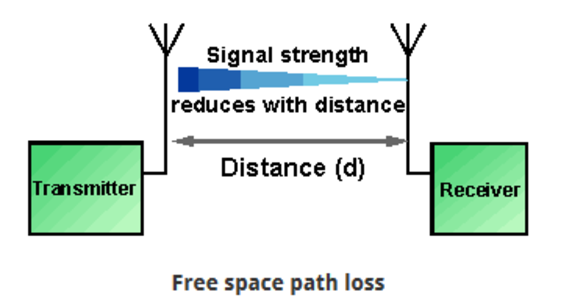
\includegraphics[width=0.6\textwidth]{freespace_fig.pdf}
%\caption{Illustration of Near field and Far field \citep{farnear_field}}
%\label{para_wave}
%\end{figure}


\section{Two Ray Plane Earth}
In contrast to the Friss pathloss model, the Two-ray-ground-reflection path loss model \citep{two_ray}, considers both the direct wave and the reflected ground wave. Also the Two-ray-ground-reflection path loss model does not depend on the frequency, as the Friss pathloss model does. The received power depending on the distance is given in the following Formula:

\begin{equation}
P_r(d) = \frac{P_t G_t G_r h^2_t h^2_r}{L \cdot d^4}
\label{two_ray_model}
\end{equation}

Where $h^2_t$ and $h^2_r$ are the heights of the transmitter and receiver antennas respectively. And L is the system loss. 

If the distance $d$ is less then a critical point $d_{c}$: 

\begin{equation}
d<d_{c}
\label{two_ray_cond}
\end{equation}

Where $d_{c}$ is given as:

\begin{equation}
d_{c} = \frac{4\pi \cdot h_t h_r}{\lambda}
\label{critical_fac_dc}
\end{equation}

If this condition is true then the two-ray model shall not give good results due to oscillations which are caused by the constructive and destructive combination of the two rays. This condition is true for small distances $d$.

%else will the received power theoretically oscillates between
%local maxima of 6dB above free space to $-\infty$ dB at local minima.

%\subsubsection{Power vs distance} 

%\subsubsection{Propagation path}

%The path can be divided into three segments the first being if:

%\begin{equation}
%d<h_{t}
%\end{equation}

%If this condition is true then:

%\begin{itemize}
%The two rays add constructively
%Path loss is slowly increasing 
%\end{itemize}




%LPE = 40 log10(d) $-$ 20 log10(ht) $-$ 20 log10(hr )

\citep{1GMSK}


%% literaturliste og bilag %%
\bookmarksetup{startatroot}% this is it
\addtocontents{toc}{\bigskip}% perhaps as well
\bibliography{setup/mybib}
\label{bib:mybiblio}
 
 \newpage
 \fancyhead[RO]{\small Appendix \nouppercase\rightmark} %even page - chapter title
 \fancyhead[LE]{\small Appendix \nouppercase\rightmark} %uneven page - section title
\fancyhead[RE,LO]{}
 \titleformat{\section}[hang]{\Large\bfseries}{\thesection\hsp\textcolor{black}{|}\hsp}{0pt}{\Large\bfseries}

 \renewcommand{\thesection}{\Alph{section}}
 \setcounter{section}{0}




\chapter*{Appendix}
 \addcontentsline{toc}{chapter}{Appendix}
 \addtocounter{chapter}{1}


\end{document}